\chapauth{Part of Everything}
\chapter{The Death Hamsters}





Luke Bavarious strolled calmly through the mall, one hand
absentmindedly stroking the cold metal of the trusty Baretta in his
pocket. ``I need a pet,'' he thought, and he made a beeline for the
pet store at the end of the strip.



Suddenly a little boy sitting on a mall bench yelled out. ``Hey
mister! I don't think you should go in there,'' he hollered.



Luke squinted at the boy and drew closer. ``Why not?'' he
inquired.



The boy looked all around and then whispered in a hoarse voice, ``I
saw a man go in there earlier. He looked insane. He had a bag full
of something lumpy. I didn't trust him. He came out without the
bag. Nobody has come out since.''



Luke laughed. ``Balderdash,'' he chuckled, and strolled off towards
the pet store. The boy slumped in his seat with a frown.



Luke walked in through the door and the door chime beeped to signal
that a person had entered. He looked around and there was no one
but he didn't really care. He knew someone would come up when he
needed to make a purchase.



He tried to decide what kind of pet to get. There were dozens of
animals. He looked at some fish and then sadly shook his head. ``Too
watery,'' he muttered to himself, and moved on. There were some
green lizards there. They stuck to the glass with their toes and he
was fascinated at this miracle of God. But he decided against it
because they might decide to stick to him and then what would he
do.



He saw puppies and kittens that were so cute that Luke choked back
a sob of joy. He had had a puppy when he was a little boy but one
day a burglar was running through his backyard where the puppy was
playing. The burglar was evil and the puppy was in his way. He
picked up the puppy and twisted it in half and then threw the
bottom half against Luke's window while he was sleeping. Luke woke
up screaming and barfed. He had never forgotten that day. He wiped
away tears thinking about it.



He decided he wanted a hamster. They were so cute. The clerk had
not shown up yet and he began to wonder. He looked all around but
couldn't find her. Then he saw the door at the back was open a bit.
So he went there and when he looked he saw a sight that made him
scream very loudly.



The mangled corpse of the clerk was lying on the floor. There was
guts everywhere. She was covered with bloody hamsters. They were
evil hamsters and they were eating her like piranhas not in
water.



With shaking hands Luke drew his Baretta. He was ready to shoot but
then something soft landed on him. ``What the'' he said and looked
over his shoulder and he saw what he thought was a pom pom. But it
wasn't. It was a hamster. Then another one landed on his other
shoulder and 2 more on his head. Then they hissed and lunged.
``Hhh,'' Luke screamed as they ate his face.



A superhuman strength came over him then and he flung all of them
off. He shot some but there were too many. He could hardly see
because his eyes were full of blood. He tripped over a bag of dog
food and then he got an idea. He pulled his lighter out of his
pocket and lit the bag of food. It went up in flames and blocked
the hamsters. The hamsters shrieked and burned. Luke took his
chance and ran out.



The boy was waiting there, still on his bench. ``I told you,'' he
yelled at Luke. ``Something was weird. You should have
listened!''



Luke stumbled over to the boy. ``I'm so sorry,'' he choked. ``I should
have respected you. Listened to you. I didn't because you're only
10 years old. I was wrong.'' He pulled a chocolate bar out of his
pocket and gave it to the boy. The boy looked at him with a big
smile and shining eyes and was happy.



By then the police were there. One of them pinned a medal on Luke's
chest. ``You're a hero, son,'' he said in a deep voice with emotion.
``There was an insane man who put evil hamsters in the store. He's
in jail now. You stopped them from killing us all.''



Luke was proud. That night he was in the paper.



\begin{figure}[b]
  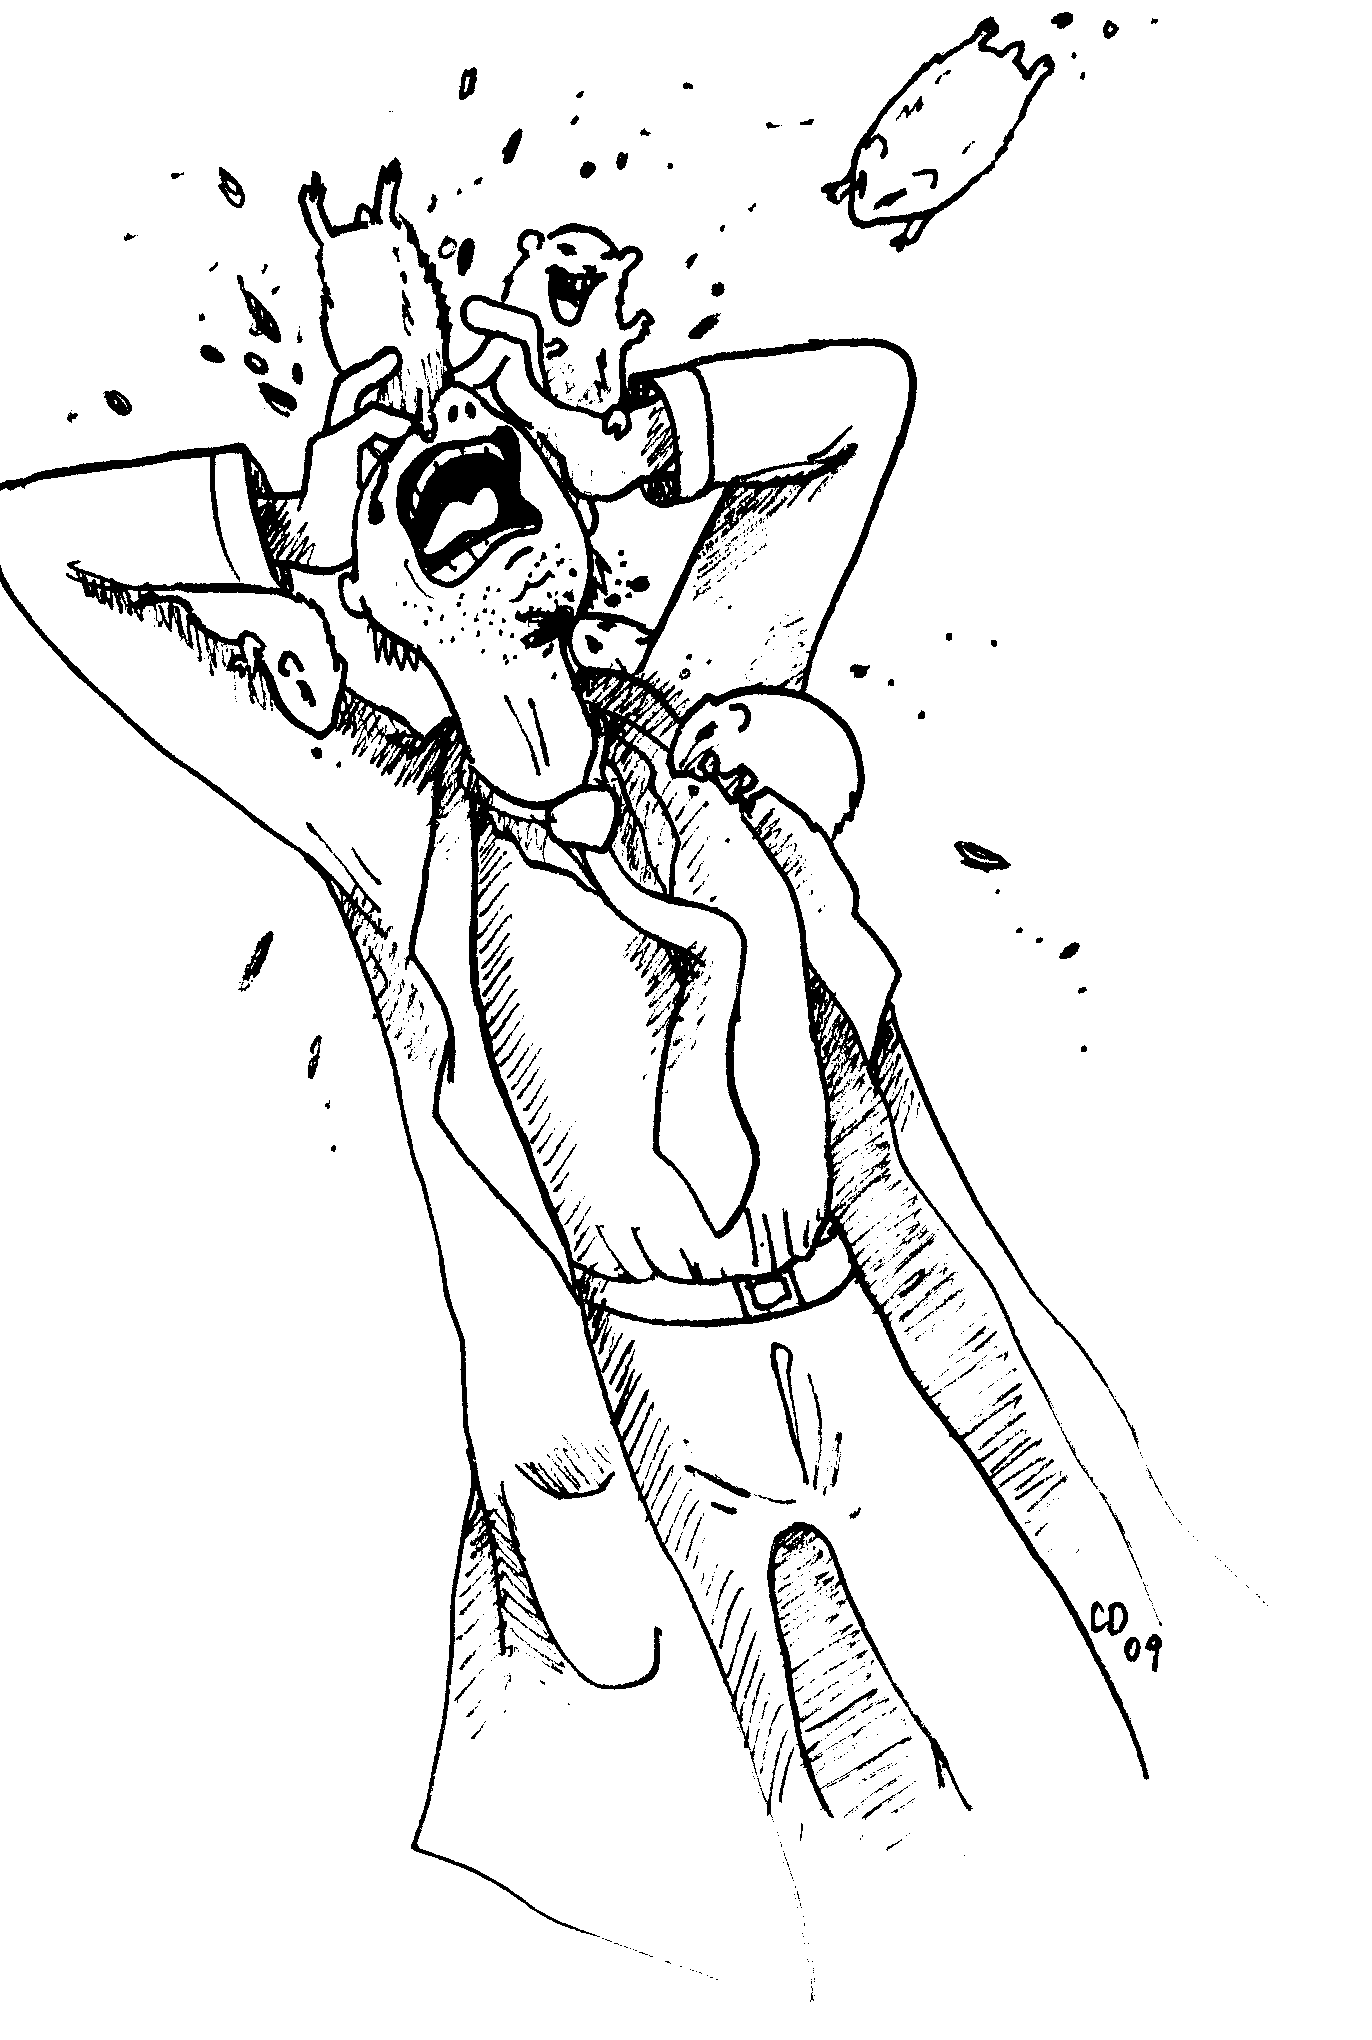
\includegraphics[width=\textwidth]{art/Part_of_Everything-Death_Hamsters.png}
  \caption{Artwork by Part of Everything}
\end{figure}
